\chapter{Implementierung}\label{ch:implementation}



%Für unsere Implementation wird für das Zwischenspeichern von Daten ein Serviceworker eingesetzt. Serviceworker können wie ein Proxy zwischen dem Webbrowser und dem Webserver agieren, welcher die Webseite bereitstellt. Stellt ein Browser eine Anfrage, so wird diese vom Serviceworker abgefangen. Der Serviceworker schaut zunächst in seinem Cache, der sog. IndexDB, ob er die gestellte Anfrage beantworten kann. Ist dies nicht der Fall, so wird die Anfrage an den Webserver weitergeleitet. Wird die gleiche Anfrage nochmals gestellt, kann diese aus dem Cache beantwortet werden, da gestellte Anfragen eine gewisse Zeit lang zwischengespeichert werden.
%\begin{figure}[!h]
%	\centering
%	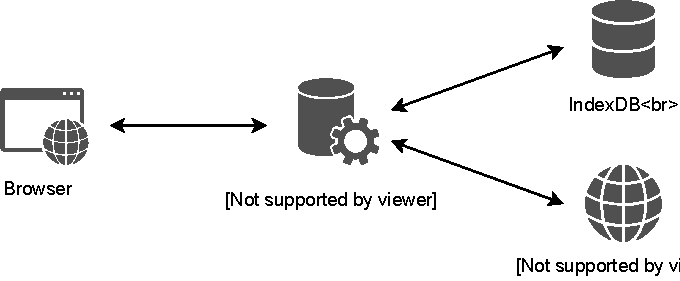
\includegraphics[width=0.8\textwidth]{figures/ServiceWorker}
%	\caption[A Figure Short-Title]{A Figure Title}
%	\label{fig:sequenceDiagram}
%\end{figure}
%
%
%Die von uns eingesetzte Technologie zur Übertragung von Daten zwischen Browsern ist WebRTC. WebRTC ist ein offener Standard und ermöglicht es Browser paarweise zwecks Datenaustausch zu verbinden. Der große Vorteil dieser Technologie ist, dass sie direkt von modernen Browsern unterstützt wird, wodurch keine zusätzliche Software installiert werden muss. Konkret wird von uns ein sog. DataChannel genutzt.
%
%Für den Datenaustausch müssen wechselseitig DataChannel zueinander aufgebaut werden. Die Ausgangslage ist, dass die Schüler wissen, dass es den anderen gibt, aber nicht wie der jeweils andere zu erreichen ist. Um diese Problematik zu lösen, existiert ein Vermittlungsserver (Signaling server).
%
%Als erstes werden Informationen, über die Verbindung die aufgebaut werden soll, an den Signaling server gesendet. Technisch wird ein SDP-offer gesendet, wobei SDP für Session Description Protocol steht. Dieses SDP-offer leitet der Signaling server an die Schüler in der Klasse/Schule weiter. Geantwortet wird mit einer SDP-answere, welche Informationen über die abgestimmte Verbindung enthält und über den Signaling server zurück geleitet wird.
%
%Damit eine direkte Verbindung aufgebaut werden kann, müssen über den Signaling server noch weitere Informationen wie ICE-Kandidaten ausgetauscht werden. ICE steht hierbei für Interactive Conectivity Establishment und ist fester Bestandteil von WebRTC. Es ist für den Aufbau der Browser-zu-Browser-Verbindung verantwortlich. ICE-Kandidaten enthalten hauptsächlich Informationen darüber wie ein bestimmter Nutzer erreichbar ist (also z.B. private oder öffentliche IP-Adresse). Ermittelt werden diese ICE-Kandidaten mithilfe eines STUN-Servers und dem dazugehörigen Session Traversal Utilities for NAT (STUN) Protokoll. Wie der Name des Protokolls schon verrät, wird es vor allem benötigt um auch Nutzer erreichen zu können die keine eigene öffentliche IP-Adresse besitzen, bei denen also Network address translation (NAT) eingesetzt wird. Dies ist aufgrund der mangelnden Anzahl an IPv4-Adressen bei fast jedem Internetnutzer der Fall.
%
%In dem Signaling server selbst wird die Logik abgebildet, wie die Klassen und Schüler miteinander in Verbindung stehen. Implementiert wurde dieser mit socket.io, da die native Klassenorganisation und Websocket-Technologie sich nahezu perfekt für unser Szenario anbot.

\section{Architectur}

\begin{itemize}
  \item Technologiewahl
  \item ES6 compilation
  \item Beschreibung der Komponenten:
  \item Service Worker
  \item 	Cached Ressourcen
  \item 	Proxy
  \item P2PCDN
  \item 	Schnittstelle für externe Anwendungen
  \item 	Nimmt Konfiguration entgegen
  \item 	Initialisiert CDN
  \item Middleware
  \item 	Vermittler zwischen Service Worker und Script
  \item 	Arbeitet mit Events
  \item 	Welche Events gibt es wer registriert sich drauf?
  \item Peer
  \item 	Representiert eigenen Peer
  \item 	Hält verbindungen zu anderen Peers
  \item Signaling
  \item FayeConnection	
\end{itemize}

\begin{figure}[!h]
	\centering
	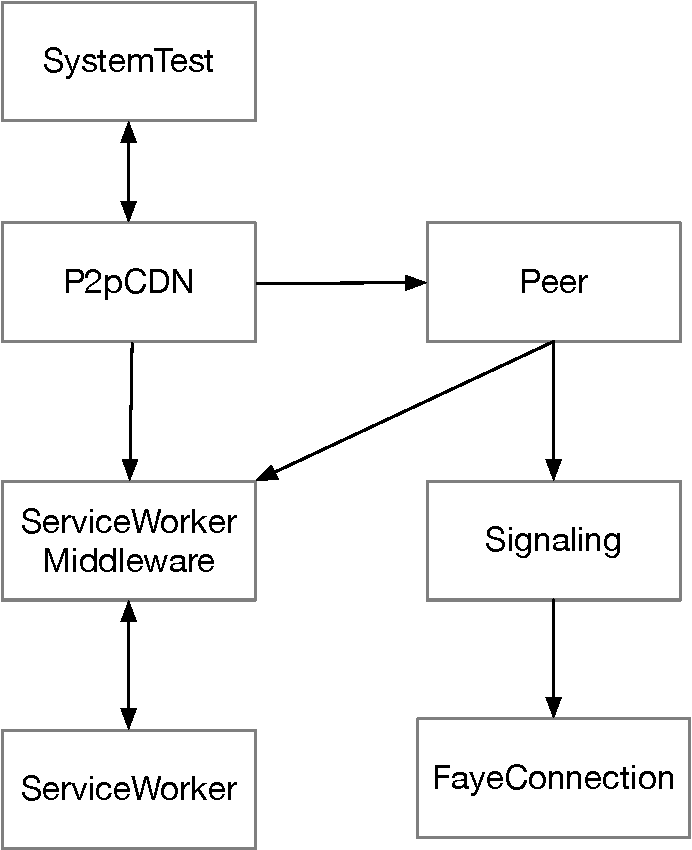
\includegraphics[width=0.8\textwidth]{figures/Klassendiagramm}
	\caption[A Figure Short-Title]{Klassendiagramm}
	\label{fig:Klassendiagramm}
\end{figure}


\subsection{Service worker}

\begin{figure}[!h]
	\centering
	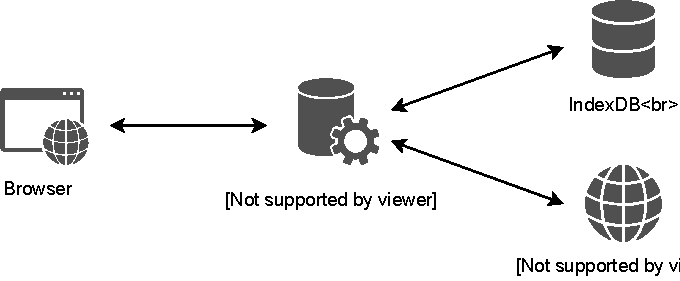
\includegraphics[width=0.8\textwidth]{figures/ServiceWorker}
	\caption[A Figure Short-Title]{A Figure Title}
	\label{fig:sequenceDiagram}
\end{figure}
\begin{itemize}
  \item warten bis sw active ist/alle verbindungen ready sind vs request normal durchgehen lassen bis alles fertig ist.
  \item 	Austausch erst möglich wenn script geladen ist
  \item 	blockent: 
  \item 		Ressourcen werden so lange aufgehalten bis verbindung initialisiert
  \item 		--> längere Ladezeiten
  \item 		mehr Bandbreite kann gespart werden
  \item 	nicht blockent: 
  \item 		Ressourcen werden über server geladen bis verbinungen aufgebaut sind
  \item 		Weniger Bandbreite wird gespart
  \item 		Ladezeit wird nicht verzögert
  \item 		Heartbeat um zu überprüfen ob script geladen ist
  \item Mehrere Tabs?
  \item 		
  \item first page load
  \item Single page apps
  \item Turbolinks
  \item Requests werden erst nach erfolgreicher registrierung behandelt
  \item clients.claim + skip waiting für den ersten aufruf (12)
  \item Codebeispiel für wartende messages
  \item 	Callbacks
\end{itemize}

\subsection{Tests}

\begin{itemize}
  \item mocha
  \item chai
  \item karma
  \item event handler testen
  \item registrieren/abmelden --> test helper
\end{itemize}

%- mocha
%- chai
%- karma
% Event handler testen
% 	- registrieren/abmelden --> test helper

\section{Ressourcen Management}



\section{Configuration}

\begin{itemize}
	\item id
	\item id length
	\item beispiel
	\item verbose
	\item ...
	\item Config Übergabe zu Service worker über IndexedDB
	\item Script lädt Config in indexedDB
	\item Service worker lädt config falls noch keine vorhanden ist und im activate event	
\end{itemize}

\subsection{Quota limits - Löschen von Requests aus dem Cache}

\begin{itemize}
  \item benötigte speichermenge wird geschätzt
  \item headersize plus 'Content-Length' header wert
  \item solange löschen bis genug speicher frei ist
  \item Quotas flexibel
	\item Quota kann abgefragt werden
	\item Quota für browser nicht für page
	\item berechnung der größe schwer
	\item löschen des ersten Elements im Cache
	\item evtl verschiedene verfahren diskutieren
	\item Fehlerfall muss abgefangen werden
\end{itemize}

\section{Client UI Events}
\begin{itemize}
	\item Events um die einbindende Anwendung über neue/gelöschte Peer Verbindungen zu informieren
	\item ui:onUpdate
\end{itemize}
\section{Signaling Server}
The signaling server itself uses socket.io and can be found here. The client ID is created there and is essential for the lifecycle of a peer in the whole network. It is not clear if the client IDs given by socket.io always have the same length. Therefore, client IDs will be padded to a maximal length of 24. This is necessary because the client IDs need to be sent via the binary datachannel and consequently, this requires a fixed length.


\begin{itemize}
  \item websockets faye
  \item gleicher data channel zur Bildung von meshs
  \item ID pro client
  \item max id length muss festgelegt werden für chunking
  \item Protokoll von P2PCDN umgesetzt
  \item Protokoll erklären
  \item Diagram Protokoll
  \item Peer Meshing wird von anwendung übernommen
\end{itemize}

\subsection{Slidesync}
\begin{itemize}
	\item Rails Model
	\item Code Beispiel
	\item Tracking in Redis welcher Peer in welchem Submesh ist
	\item Peer wird aus liste nicht voller mehses gewählt
	\item Falls alle voll sind wird neues Mesh angelegt und garbage collection gestartet.
	\item Datentyen und mapping erklären
	\item Background job räumt leere meshes auf (Garbage collection)
	\item 	löscht leere meshes aus liste
\end{itemize}

\subsection{\schulCloud}

\section{Message protocol}
%In unserer Implementation wird, sobald eine neuer Besucher der Webseite hinzukommt, sofort ein DataChannel, mittels WebRTC, STUN, ICE und Signaling server zu allen anderen aktiven Besuchern aufgebaut. Über diesen werden zu zwei Zeitpunkten Informationen darüber ausgetauscht, welche Ressourcen bei dem jeweiligen Nutzer vorliegen: Direkt nach Aufbau des DataChannels und immer dann, wenn ein Nutzer eine neue Ressource (aus dem Internet oder lokal) geladen und in seinem Cache gespeichert hat:

\begin{figure}[!h]
	\centering
	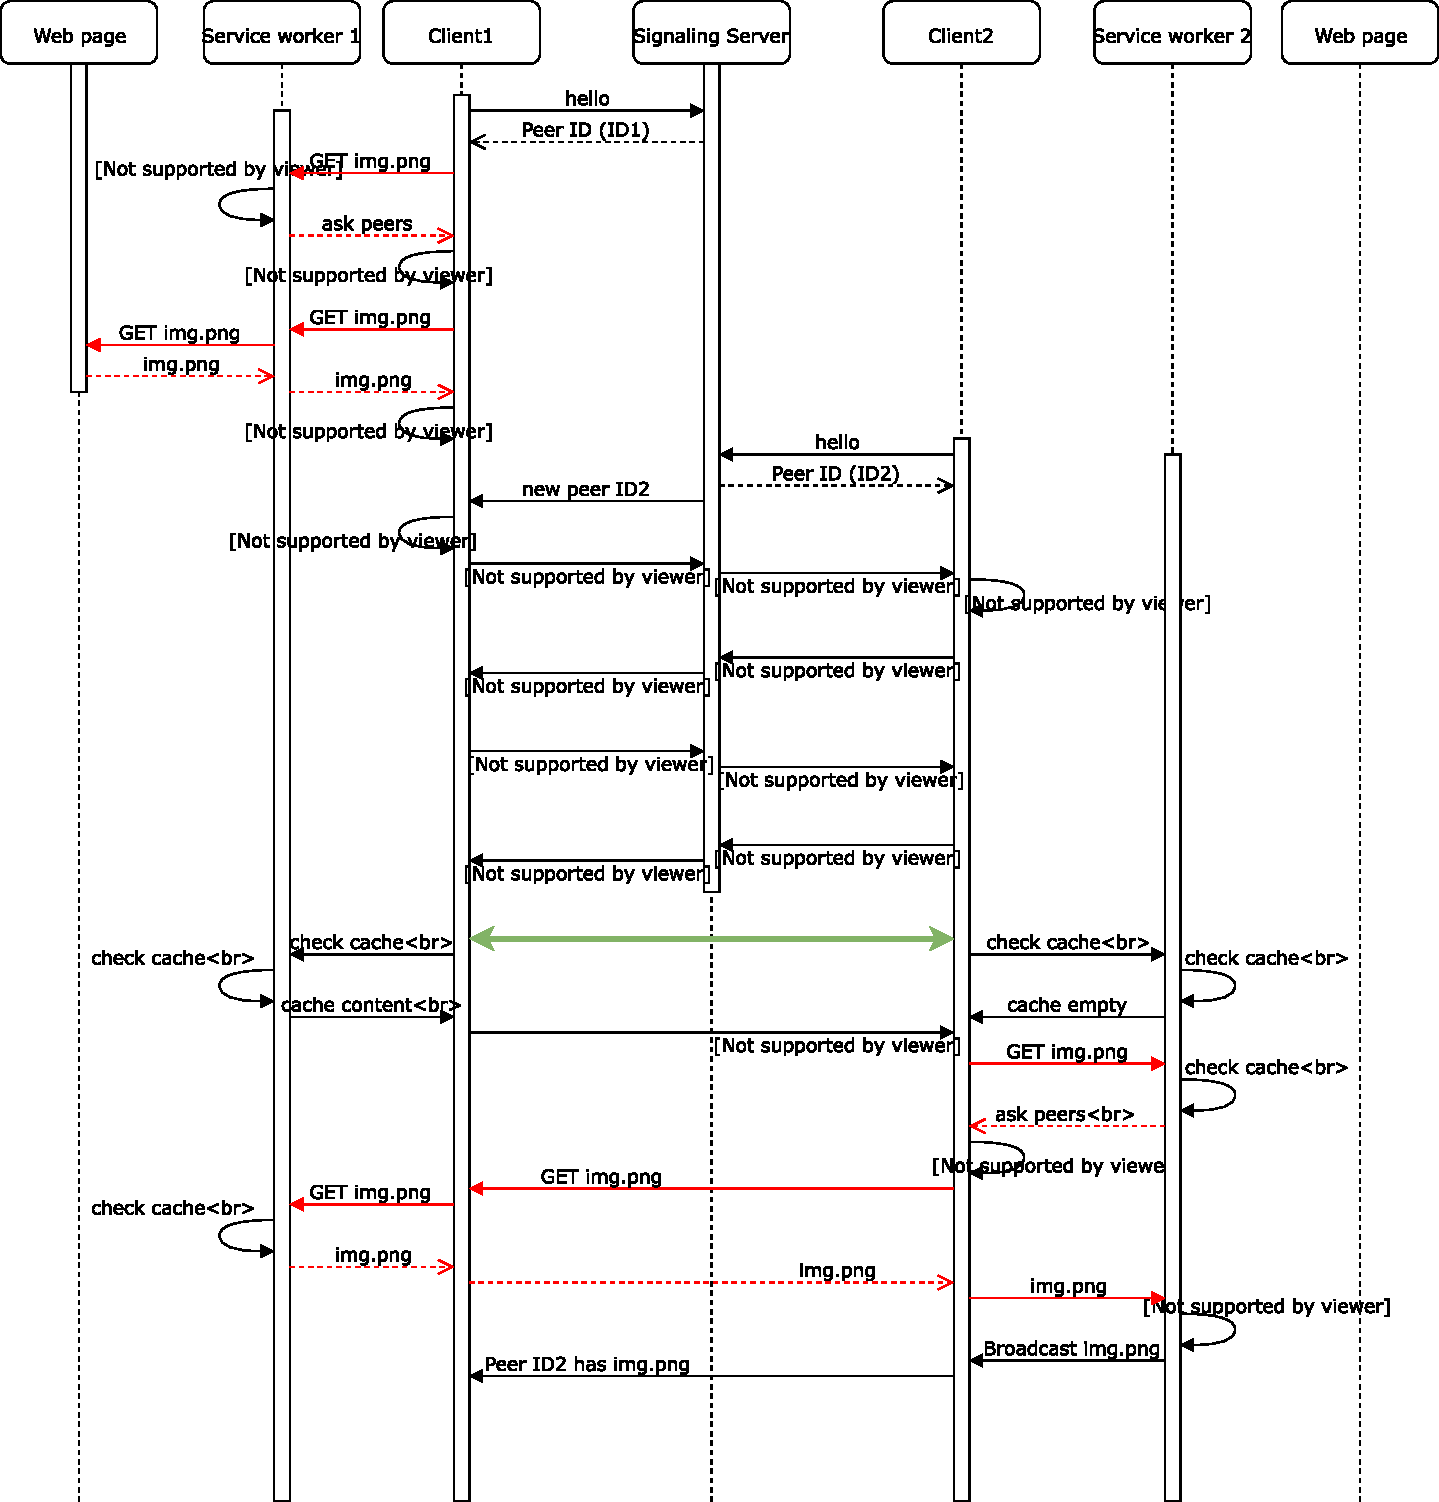
\includegraphics[width=0.8\textwidth]{figures/SequenceDiagram}
	\caption[A Figure Short-Title]{A Figure Title}
	\label{fig:sequenceDiagram}
\end{figure}
\todo{Diagramm aktualisieren}

%Client 1 (C1) ist der erste der die Webseite aufruft. Er registriert sich beim Signaling server und fragt im Anschluss img.png an (rot). Da noch niemand anders auf der Seite ist von dem er die Ressource bekommen könnte und er zudem die Ressource nicht in seinem Cache hat, wird img.png über das Internet vom Webserver geladen. Client 2 (C2) ruft nun ebenfalls die Webseite auf und registriert sich beim Signaling server. Dieser benachrichtigt C1, dass ein neuer Teilnehmer registriert wurde, woraufhin C1 einen Verbindungsaufbau zu C2 einleitet. Steht die direkte Verbindung zwischen C1 und C2 (grün), teilt C1 C2 den Inhalt seines aktuellen Caches mit. Fragt C2 img.png an (rot), weiß er so, dass er diese von C1 anfragen kann. Hat er img.png erhalten, teilt er allen anderen Teilnehmern (in diesem Fall nur C1) mit, dass auch er jetzt img.png als Ressource in seinem Cache hat

\subsection{Updates}
\begin{itemize}
	\item message types
	\item neue Resource
	\item gelöschte Resource
	\item Client tritt dem Netzwerk bei
	\item Client verlässt Netzwerk
	\item Diagram aktualisieren
	\item alle Clients müssen benachrichtigt werden
	\item Über Webrtc data channel
	\item Message format zeigen
\end{itemize}
\subsection{Client fragt Ressource an}
\begin{itemize}
	\item Message Format
	\item Diagram beschreiben
\end{itemize}
\section{Mesh Zuordnung}
% data Channels zur mesh verbindung definiert über Anwendung
% ip subnetz erkennung wie implementiert?

\section{Reusability}

\section{Serialisierung der Daten}
Für den Austausch von Daten werden die von WebRTC angebotene DataChannel genutzt, welche das Stream Control Transmission Protocol kurz SCTP verwendet. Problem hierbei ist, dass dieses Protokoll ursprünglich für die Übertragung von Kontrollinformationen designt wurde und deshalb für die Kompatibilität verschiedener Browser eine Paketgröße von 16kiB nicht überschritten werden sollte. In unserem Kontext ist es aber notwendig auch größere Dateien zu übertragen, weshalb aktuell viele kleine Datenpakete verwendet werden müssen. Hierdurch entsteht ein nicht zu vernachlässigender Overhead.
\begin{itemize}
  \item SCTP(DataChannel) message size limit 16kiB
  \item chunking reassembling nötig
  \item Performance einbussen
  \item abToMessage und sendToPeer
\end{itemize}

% SCTP(DataChannel) message size limit 16kiB
% chunking reassembling nötig
% _abToMessage() und _sendToPeer
% Performance einbußen

%Currently, it is only possible to send messages not larger than 16kiB via the RTCDataChannel. In order to send larger messages chunking and reassembling is necessary. These procedures take place in the _abToMessage() and _sendToPeer() methods in the peer.js file.

\begin{itemize}
	\item Details zum Algorithmus
\end{itemize}
\section{System Test}
\begin{itemize}
	\item Browser Support
	\item 	modernizer
	\item 	testet auf Browserversion
	\item Test von Verbindungsaufbau
	\item 	mit anderen Clients verbunden?
	\item Code Beispiel verwendung des Interfaces
\end{itemize}

\section{Erfassen von Statistiken}
\begin{itemize}
	\item Client Script sendet an Service Worker von wem etwas geladen wurde
	\item Service Worker trackt wie Request abgearbeitet wurde
	\item Service Worker sendet periodisch alle Metadaten an Server
	\item Server trackt statistiken
	\item Fall Slidesync:
	\item 	Live statistik tracking
	\item 	evtl. Mongo db
	\item 	anzeigetool
\end{itemize}

\section{Storage quotas}
\begin{itemize}
	\item Wichtig um fehlervorzubeugen
	\item Browser besitzt dynamische Quotas, abhänig von 
	\item Quoata für CDN kann über einstellungen festgelegt werden.
	\item navigator.storage.estimate()
	\item Quota Management API
	\item 	LRU falls quota erreicht
	\item 	Löscht kompletten Cache für eine Seite
	\item https://developers.google.com/web/updates/2017/08/estimating-available-storage-space
	\item https://developer.mozilla.org/en-US/docs/Web/API/IndexedDB_API/Browser_storage_limits_and_eviction_criteria
	\item Eigene Implemtierung
	\item 	Round Robin
	\item 	Größe des Requests wird geschätzt
	\item 	Exakte größe schwer berechnen bar da cache komprimiert
	\item 	Größe des Kontents plus größe des Headers plus offset
	\item 	Cache wird geleert bis genug platz frei ist.
\end{itemize}


\begin{listing}[h]
	\inputminted{ruby}{listings/context-data-transform.rb}
	\caption{Some Code Snipped}
	\label{lst:code-snipped}
\end{listing}

\section{Resource loading}
